\newpage
\section*{Annexe}
\subsection*{Options de migration}
Qemu propose certaines optimisations pour aider la migration à ce dérouler d'une manière plus efficace en terme du volume des données transférer et ainsi avoir le temps d'absence de la machine virtuelle le plus faible possible sans impacter les performances de cette dernière.

\subsubsection*{Xor Based Zero Run Length Encoding}
La capability xbzrle a pour but de réduire le downtime ainsi que le temps total de la migration.
Elle est utile s'il existe sur la machine virtuelle des processus qui font des accès mémoire intensive.
Quand cette option n'est pas activée, la totalité de la mémoire serra transférée.
Cette technique a pour but de chercher les changements en mémoire qui ont été faits depuis la dernière itération de la transmission de la mémoire, les compresser, et les transmettre à la machine destination.
ce qui permet de réduire le volume des données transférées entre les deux bout de la communication.

Pour pouvoir trouver les zones en mémoire qui ont changé, la VM émettrice doit garder l'ancien état de la page dans un cache
avec un algorithme d'éviction LRU (la taille par default du cache est de 64 Mo), puis xbzrle encode le delta entre
les deux pages.
Du côté de la VM réceptrice, elle utilise le contenu de la dernière page reçu et xbzrle pour décoder le nouveau contenu de la page.

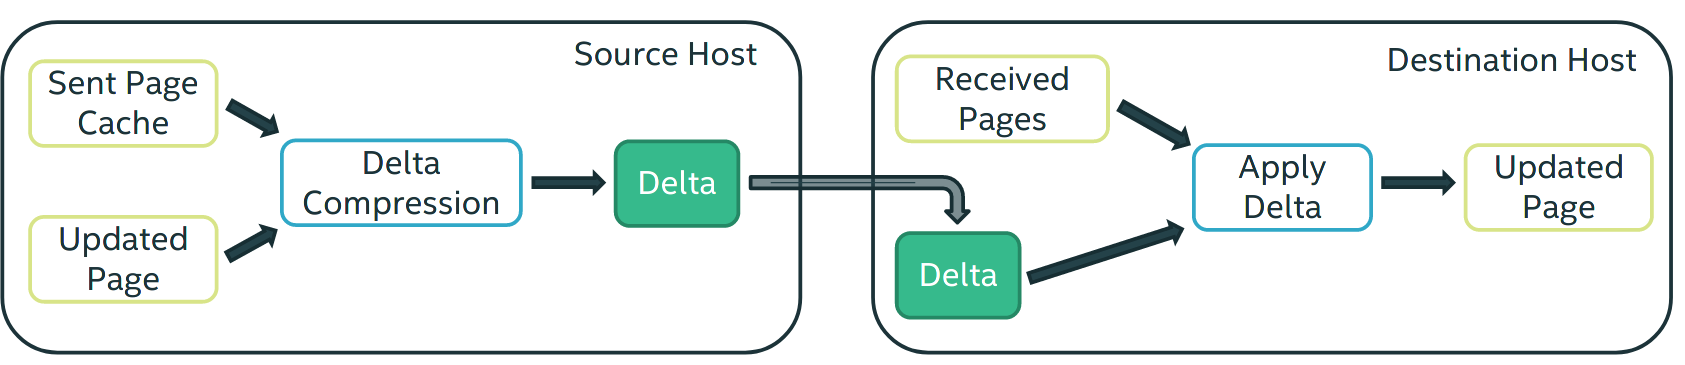
\includegraphics[width=\textwidth]{include/xbzrle}
Le delta est calculé avec un xor entre l'ancien et le nouveau contenu de la page, le résultat de ce xor est des suites de zéros et d'uns,
ces derniers sont compressés de la manière suivante:

\begin{itemize}
    \item une suite de zéros est représentée par sa taille.
    \item une suite d'uns est représentée par sa taille suivie des nouvelles données.
    \item la taille est encodée avec ULEB128.
\end{itemize}
\subsubsection*{Paramètres}
\begin{itemize}

 \item[$\bullet$]xbzrle-cache-size: Taille du cache utilisé par XBZRLE lors de la migration, il doit être multiple de la taille de la page cible et une puissance de 2.

\end{itemize}

source:  \url{docs/xbzrle.txt}

\subsubsection*{Compress}
La capability compress a pour but de réduire la taille des données transférées pendant la migration.
Cette option consiste à compresser chaque page de RAM avant de l'envoyer sur le réseau, du côté
réception la page serra décompressé pour restaurer les données d'origine.
Cela peut être utile si on a une bande passante limitée.
En compressant les pages, on peut s'attendre à réduire de 60\% des données transférer
ainsi que réduire le temps total de migration et le downtime respectivement de 70\% et 50\%.

Le point négatif de cette approche, c'est qu'on augmente drastiquement le temps CPU dus au thread de compression et de décompression.
et donc augmenter le temps de migration. Si l'on possède un algorithme de compression assez performant, on peut réduire le temps de migration en augmentant le nombre thread
Cette option consomme beaucoup de temps CPU dans un système ou le CPU est le bottleneck il faudrait plutôt l'éviter, par contre
sur un système ou la bande passante est faible et le CPU est adéquat il est plus préférable d'utiliser la compression sur plusieurs threads.
\newline
\newline
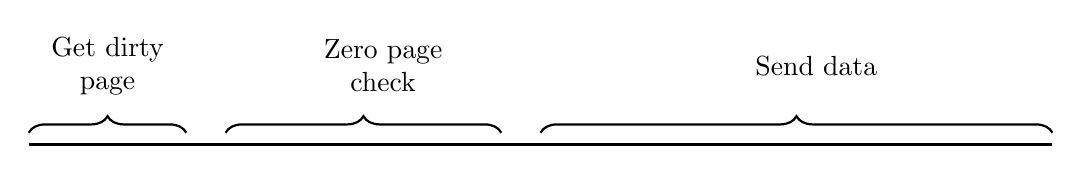
\begin{tikzpicture}[scale=1]
    \node[align=center] at (1,1) {Get dirty \\ page};
    \draw [thick,decorate,decoration={brace,amplitude=6pt,raise=0pt}] (0,0.15) -- (2,0.15);

    \node[align=center] at (4.5,1) {Zero page \\check};
    \draw [thick,decorate,decoration={brace,amplitude=6pt,raise=0pt}] (2.5,0.15) -- (6,0.15);

    \node[align=center] at (10,1) {Send data};
    \draw [thick,decorate,decoration={brace,amplitude=6pt,raise=0pt}] (6.5,0.15) -- (13,0.15);

    \draw [thick,-] (0,0) -- (13,0);

\end{tikzpicture}
\captionof{figure}{Sans (dé)compression.}

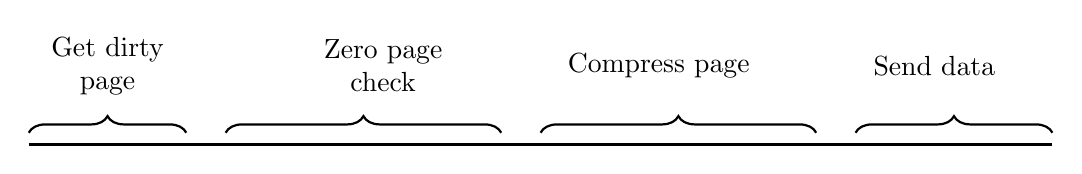
\begin{tikzpicture}[scale=1]
    \node[align=center] at (1,1) {Get dirty \\ page};
    \draw [thick,decorate,decoration={brace,amplitude=6pt,raise=0pt}] (0,0.15) -- (2,0.15);

    \node[align=center] at (4.5,1) {Zero page \\check};
    \draw [thick,decorate,decoration={brace,amplitude=6pt,raise=0pt}] (2.5,0.15) -- (6,0.15);

    \node[align=center] at (8,1) {Compress page};
    \draw [thick,decorate,decoration={brace,amplitude=6pt,raise=0pt}] (6.5,0.15) -- (10,0.15);

    \node[align=center] at (11.5,1) {Send data};
    \draw [thick,decorate,decoration={brace,amplitude=6pt,raise=0pt}] (10.5,0.15) -- (13,0.15);

    \draw [thick,-] (0,0) -- (13,0);

\end{tikzpicture}

\captionof{figure}{Avec (dé)compression.}

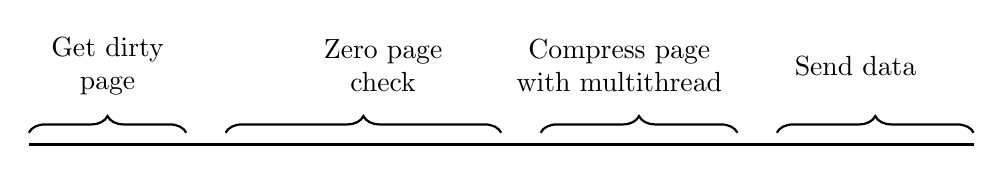
\begin{tikzpicture}[scale=1]

    \node[align=center] at (1,1) {Get dirty \\ page};
    \draw [thick,decorate,decoration={brace,amplitude=6pt,raise=0pt}] (0,0.15) -- (2,0.15);

    \node[align=center] at (4.5,1) {Zero page \\check};
    \draw [thick,decorate,decoration={brace,amplitude=6pt,raise=0pt}] (2.5,0.15) -- (6,0.15);

    \node[align=center] at (7.5,1) {Compress page\\with multithread};
    \draw [thick,decorate,decoration={brace,amplitude=6pt,raise=0pt}] (6.5,0.15) -- (9,0.15);

    \node[align=center] at (10.5,1) {Send data};
    \draw [thick,decorate,decoration={brace,amplitude=6pt,raise=0pt}] (9.5,0.15) -- (12,0.15);

    \draw [thick,-] (0,0) -- (12,0);

\end{tikzpicture}

\captionof{figure}{Avec multi-thread (dé)compression.}


\subsubsection*{Paramètres}
\begin{itemize}

    \item[$\bullet$] compress-level: Niveau de compression:
        \begin{itemize}
            \item niveau 0: Pas de compression.
            \item niveau 1: Meilleure vitesse de compression.
            \item niveau 9: Meilleur ratio de compression.
        \end{itemize}

    \item[$\bullet$] compress-threads: Nombre de thread de compression.
    \item[$\bullet$] decompress-threads: Nombre de thread de décompression.
    \item[$\bullet$] compress-wait-thread: Donne la démarche à suivre si tous les thread de compression sont utilisés, Si à true (par défault), il faudra attendre qu'un thread devienne libre; sinon, on envoie la page sans compression.
\end{itemize}

source:  \url{docs/multi-thread-compression.txt}

\subsubsection*{Auto converge}
Certains workload ont tendance à salir la mémoire plus rapidement que le taux de transfert.
Malgré quelques améliorations récentes (et l'utilisation de cartes réseau 10Gb entre les hôtes) la migration peut ne pas converger.
\\

Pour résoudre ce problème, l'option autoconverge permet de ralentir le CPU en interdisant
explicitement aux VCPU de passer beaucoup de temps dans la VM, cela permet de valider la condition de passage
à la phase 3 de la migration plus rapidement (phase d'arrêt).

\subsubsection*{Paramètres}
\begin{itemize}
    
 \item[$\bullet$]throttle-trigger-threshold: Le ratio entre bytes\_dirty\_period et bytes\_xfer\_period
                              pour activé la dégradation des performances.
                              Valeur par défault est de 50 (pourcentage).

 \item[$\bullet$]cpu-throttle-initial: Le pourcentage initial de la dégradation des performances si auto-converge est activé.


 \item[$\bullet$]cpu-throttle-increment: L'increment du pourcentage des performence à reduire si on voit que la migration ne converge pas.

 \item[$\bullet$]max-cpu-throttle: Pourcentage maximum de la dégradation, par défault à 99.
\end{itemize}

source:  \url{https://wiki.qemu.org/Features/AutoconvergeLiveMigration}

\subsubsection*{Postcopy ram}
La Postcopy est également une méthode de migration dynamique populaire.
Par rapport à la pré-copie, la migration post-copie est plus rapide et peut presque établir une connexion transparente entre la source et la destination de la migration.
Pour les machines virtuelles avec de grandes quantités d'opérations de lecture et d'écriture de mémoire, surtout si la bande passante de migration est limitée, la post-copie est une méthode plus efficace pour la migration à chaud.

En termes simples, la post-copie consiste d'abord à transférer l'état du processeur existant, les registres et, éventuellement, la mémoire non-paginable (mémoire qui ne sera ni échangée ni déplacée en mémoire) de la machine virtuelle vers le serveur de destination.
Par la suite, la machine virtuelle est démarrée sur le serveur de destination.
Dans le même temps, le serveur source enverra également dynamiquement la mémoire restante vers le serveur de destination.
Mais lorsque la machine virtuelle utilise la mémoire qui n'a pas été transférée, une page-fault sera déclenchée.

La méthode post-copy gère ces pages-fault en se basant sur le mécanisme du noyau linux 'userfaultfd'.
userfaultfd permet à la machine cible d'obtenir les informations de la dite page via le descripteur de fichier fd dans l'espace utilisateur (espace utilisateur).
En termes simples, lorsque la machine virtuelle appelle la mémoire qui n'a pas été transférée sur le serveur de destination, userfaultfd peut accéder au serveur source pour extraire ces informations de mémoire et les transférer vers le serveur de destination pour permettre à la machine virtuelle de continuer à fonctionner.

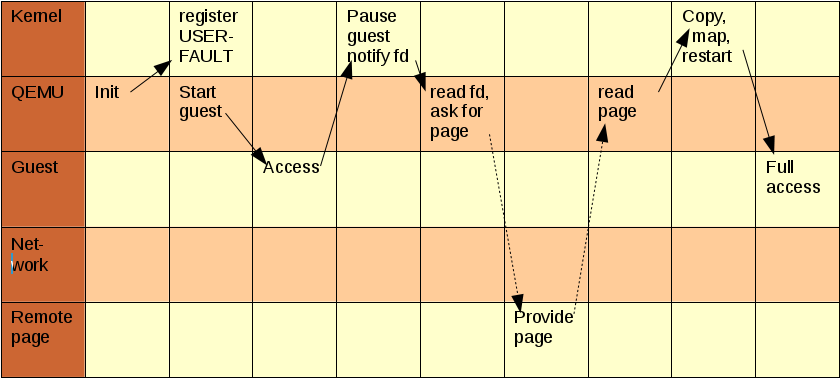
\includegraphics[width=\textwidth]{include/Postcopyflow}
\captionof{figure}{List d'appels suite à un page-fault}


La pression de lecture et d'écriture de la machine virtuelle sur la mémoire n'affectera pas le succès de la post-copie, mais une fois la migration de la machine virtuelle terminée, si la pression de lecture et d'écriture sur la mémoire est importante, userfaultfd sera appelé fréquemment, ce qui exercera une pression sur la bande passante du serveur et entraînera également une dégradation des performances de la machine virtuelle.
\\

source: 
\begin{itemize}
    \item \url{https://wiki.qemu.org/Features/PostCopyLiveMigration}
    \item \url{https://en.wikipedia.org/wiki/Live_migration#Post-copy_memory_migration}
\end{itemize}

\subsubsection*{Postcopy blocktime}
Blocktime est une métrique pour la migration en post-copy, elle montre combien de temps, le vCPU était en état de veille interruptible en raison d'une page-fault.
Cette métrique est calculée à la fois pour tous les processeurs virtuels en tant que valeur superposée et
séparément pour chaque processeur virtuel. Ces valeurs sont calculées du côté du serveur destination, elles sont utilisées pour calculer le downtime de la post-copy.

source: \url{docs/devel/migration.rst}

\subsubsection*{Multiple fds}
Cette option permet d'utiliser plusieurs fd pour procéder à la migration.
En utilisant un flux unique pour la migration, cela pose plusieurs problèmes:
\begin{itemize}
    \item Le processeur qui fait la réception est un goulot d'étranglement sur 10Gigabit et plus rapide
    \item Nous copions toutes les pages pour la migration, même lorsque nous pouvons envoyer directement
    \item Nous rendons les Transparent HugePages plus difficile à utiliser
\end{itemize}

L'idée ici est donc de diviser le flux de migration en deux, l'un pour le code actuel et l'autre pour le contenu des pages RAM. Cela évite complètement les copies.

Canal principal:
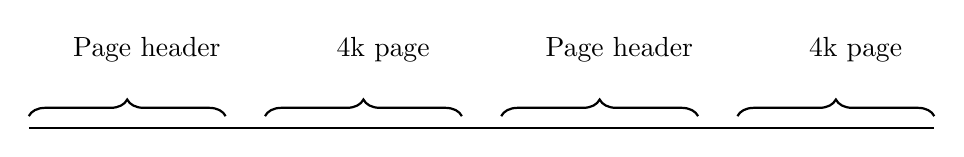
\begin{tikzpicture}[scale=1]
    \node[align=center] at (1.5,1) {Page header};
    \draw [thick,decorate,decoration={brace,amplitude=6pt,raise=0pt}] (0,0.15) -- (2.5,0.15);

    \node[align=center] at (4.5,1) {4k page};
    \draw [thick,decorate,decoration={brace,amplitude=6pt,raise=0pt}] (3,0.15) -- (5.5,0.15);

    \node[align=center] at (7.5,1) {Page header};
    \draw [thick,decorate,decoration={brace,amplitude=6pt,raise=0pt}] (6,0.15) -- (8.5,0.15);

    \node[align=center] at (10.5,1) {4k page};
    \draw [thick,decorate,decoration={brace,amplitude=6pt,raise=0pt}] (9,0.15) -- (11.5,0.15);

    \draw [thick,-] (0,0) -- (11.5,0);

\end{tikzpicture}

\captionof{figure}{Flux unique.}


Canal principal:
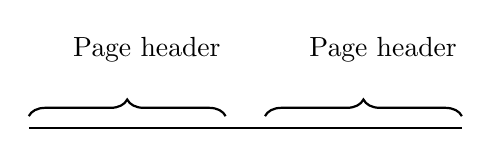
\begin{tikzpicture}[scale=1]
    \node[align=center] at (1.5,1) {Page header};
    \draw [thick,decorate,decoration={brace,amplitude=6pt,raise=0pt}] (0,0.15) -- (2.5,0.15);


    \node[align=center] at (4.5,1) {Page header};
    \draw [thick,decorate,decoration={brace,amplitude=6pt,raise=0pt}] (3,0.15) -- (5.5,0.15);


    \draw [thick,-] (0,0) -- (5.5,0);

\end{tikzpicture}


Canal secondaire:
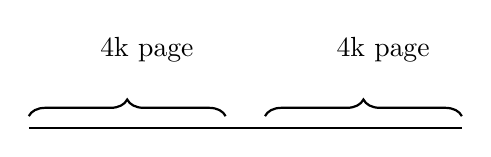
\begin{tikzpicture}[scale=1]

    \node[align=center] at (1.5,1) {4k page};
    \draw [thick,decorate,decoration={brace,amplitude=6pt,raise=0pt}] (0,0.15) -- (2.5,0.15);

    \node[align=center] at (4.5,1) {4k page};
    \draw [thick,decorate,decoration={brace,amplitude=6pt,raise=0pt}] (3,0.15) -- (5.5,0.15);



    \draw [thick,-] (0,0) -- (5.5,0);

\end{tikzpicture}

\captionof{figure}{Flux Multiple.}
\subsubsection*{Paramètres}
\begin{itemize}
 \item[$\bullet$]multifd-channels: Le nombre de flux utilisés pour la migration des données en parallèle. La par default est à 2.
\end{itemize}

source:  \url{https://wiki.qemu.org/Features/Migration-Multiple-fds}
\subsubsection*{RDMA pin all}
Le RDMA contribue à rendre votre migration plus déterministe sous forte charge, car la latence est nettement plus faible et le débit plus élevé que du TCP/IP classique, l'architecture d'E/S
RDMA réduit le nombre d'interruptions et copies de données en contournant la pile réseau hôte.

RDMA est actuellement disponible en deux versions : à la fois basée sur Ethernet (RoCE ou RDMA over Converged Ethernet) ainsi que sur Infiniband.

L'utilisation de RDMA pendant la migration nécessite de pin de la mémoire avec le matériel.
Cela signifie que la mémoire doit être physiquement présente avant que le matériel puisse transmettre cette mémoire à une autre machine.

Cette option permet d'épingler la totalité de la mémoire de la VM.



source:  \url{docs/rdma.txt}

\subsubsection*{X COLO}
Si cette option est activée, la migration ne se termine pas.
L'état du serveur émetteur serra migrer de manière constante vers le serveur destination, ce procédé est appelé COarse-Grain LOck Stepping.
c'est une technique de réplication de machine virtuelle, elle permet de fournir un «service non-stop» de tolérance aux pannes matérielles implémenté par logiciel indépendant de l'application.

La VM principale (PVM) et la VM secondaire (SVM) s'exécutent en parallèle.
Les paquets entrants du client ou du réseau externe sont reçus par le
nœud principal, puis transmis au nœud secondaire, de sorte que le PVM
et les SVM sont stimulés par les mêmes demandes.
Si les paquets de réponses de PVM et SVM sont identiques, ils sont envoyés immédiatement. Sinon, un point de contrôle VM (à la demande) est effectué.
source: \url{https://wiki.qemu.org/Features/COLO}


\subsubsection*{Autres options}
\begin{tabular}{ |p{3cm}|p{10cm}|  }
    \hline
    Nom de l'option& Description\\
    \hline
    \hline
    Zero blocks&Cette capability encode efficacement les blocs de zéros.\\
    \hline
    Release ram& Libérer les pages de RAM de la machine source migrée si l'option Postcopy ram est activée.\\
    \hline
    Block& Migrer également le contenu de tous les blocs device.\\
    \hline
    Pause before switchover& Suspendre la migration avant de sérialiser l'état des devices et avant de désactiver le block IO \\
    \hline
    Return path& La migration devra utiliser le chemin de retour même en post-copy\\
    \hline
    Dirty bitmaps& QEMU devra migrer les named dirty bitmaps\\
    \hline
    Late block activate& La destination devra ne pas activé les block devices à la fin de la migration\\
    \hline
    Ignore shared& QEMU ne va pas migrer la mémoire partagée \\
    \hline
    Validate uuid& Envoyer le UUID de la source pour permettre à la destination de vérifier la correspondance.\\
    \hline
   \end{tabular}
\\

source:  \url{https://github.com/qemu/qemu/blob/master/qapi/migration.json}
